%! Author = hxp
%! Date = 2020-11-09

\documentclass{ctexart}


\usepackage{ctex}
\usepackage{amsmath}
\usepackage{amsfonts}
\usepackage{amssymb}
\usepackage{wasysym}
\newcommand{\angstrom}{\text{\normalfont\AA}}  % 定义了原子物理的A
\usepackage{graphicx}
\usepackage{float}
\restylefloat{table}
\usepackage{geometry}
\geometry{a4paper,scale=0.8}  % 定义页面大小是A4,缩放是0.8
\usepackage{caption}
\usepackage{subcaption}
\usepackage{enumitem}

\newcommand*{\md}{\mathop{}\!\mathrm{d}}   % 定义微分算子,直立体的d
\newcommand*{\me}{\mathrm{e}}              % 定义自然对数e,同样应当是直立体

% 如果你想要每一段的开头不要空两格,注释掉下面这两行
\usepackage{parskip}
\setlength{\parindent}{0cm}

% 默认的\mathbf对希腊字母不生效,这里改下
\usepackage{bm}
\let\Oldmathbf\mathbf
\renewcommand{\mathbf}[1]{\boldsymbol{\Oldmathbf{#1}}}

% 表格默认格内内容和边框没有留出距离,显示分数的时候,分数的上下会贴到边框上
% 因此我增加了表格内容和边框的最短距离是5像素
\usepackage{cellspace}
\setlength{\cellspacetoplimit}{5pt}
\setlength{\cellspacebottomlimit}{5pt}

% \si命令是用来写单位的,单位需要和之前的数字有一个空格的距离,而且应当直立体
% 用法:5 \si{km/h}
\newcommand{\si}[1]{\mathrm{#1}}

% 日期不要显示
\date{}

\usepackage{fancyhdr}
\pagestyle{fancy}
\fancyhf{}
\lhead{本文档TeX源码地址:https://github.com/hxp-plus/Notes/tree/master/Physics-Experiment/实验报告}
\rfoot{第 \thepage 页}
\renewcommand{\headrulewidth}{1pt}
\renewcommand{\footrulewidth}{1pt}

%% 标题三号黑体,作者信息为班级姓名学号
\newcommand{\generatetitle}[6]{\title{\zihao{3}\heiti#1} \author{#2 \quad
\quad #3 \quad\quad #4 \quad\quad #5 \quad\quad #6} \maketitle\thispagestyle{fancy}}

%% 所有的引言、实验内容与数据处理啥的,用section
\ctexset {
section = {
format = \raggedright\zihao{4}\heiti,  % 设置所有section的字号为四号黑体左对齐
name={,、},                            % 序号后跟顿号
aftername={\hspace{0pt}},              % 修改序号和标题直接的间距为零
number=\chinese{section},              % 设置序号为中文
},
subsection = {
format = \raggedright\zihao{5}\heiti,  % 设置所有subsection的字号为五号黑体左对齐
number={},              % 设置序号为没有序号
},
subsubsection = {
format = \raggedright\zihao{5}\heiti,  % 设置所有subsection的字号为五号黑体左对齐
number={},              % 设置序号为没有序号
}
}

%% 实验背景、实验目的啥的,用subsection
\ctexset {
subsection = {
format = \raggedright\zihao{5}\heiti,  % 所有subsection的字号为五号黑体左对齐
number={},                             % 设置序号为没有序号
}
}

%% 把subsection之间加上中括号
\let\oldsubsection\subsection
\renewcommand{\subsection}[1]{\oldsubsection{\!\!\!\!\!\!【#1】}}
\let\oldsubsubsection\subsubsection
\renewcommand{\subsubsection}[1]{\oldsubsubsection{\!\!\!\!\!\!【#1】}}

%% 摘要和关键词用paragraph

\ctexset {
paragraph = {
format = \raggedright\zihao{5}\heiti,  % 所有paragraph的字号为五号黑体左对齐
number={},                             % 设置序号为没有序号
}
}

%% 把paragraph之间加上中括号
\let\oldparagraph\paragraph
\renewcommand{\paragraph}[1]{\oldparagraph{#1:\!\!\!\!\!\!}}

%% 再把参考文献的序号去掉
\makeatletter
\renewcommand\@biblabel[1]{}
\makeatother

\begin{document}

    \generatetitle{综合物理实验报告——
    综合光学实验}{物理4+4}{胡喜平}{U201811966}{hxp@hust.edu.cn}{https://hxp.plus/}

    \paragraph{摘要}

    \paragraph{关键词}


    \section{引言}

    \subsection{实验目的}


    \section{实验内容与数据处理}

    \subsection{实验原理}

    \subsection{实验内容}

    \subsection{实验结果的分析和结论}

\newpage
\begin{table}[H]
    \centering
    \begin{tabular}{|c|c|c|c|c|c|c|c|c|}
        \hline
        励磁电流($\si{A}$)   & 0.00 & 0.30 & 0.60 & 0.90 & 1.20 & 1.50 & 1.80 & 2.00 \\\hline
        磁场强度($\si{mT}$)  & 0.00 & 7.20 & 14.20 & 21.50 & 29.00 & 36.50 & 42.40 & 48.00 \\\hline
        反向励磁电流($\si{A}$) & 0.00 & -0.30 & -0.60 & -0.90 & -1.20 & -1.50 & -1.80 & -2.00 \\\hline
        磁场强度($\si{mT}$)  & 0.00 & -7.50 & -14.70 & -21.60 & -28.40 & -35.10 & -41.60 & -44.80 \\\hline
    \end{tabular}
    \caption{励磁电流和磁场强度关系}
\end{table}
\begin{figure}[H]
    \centering
    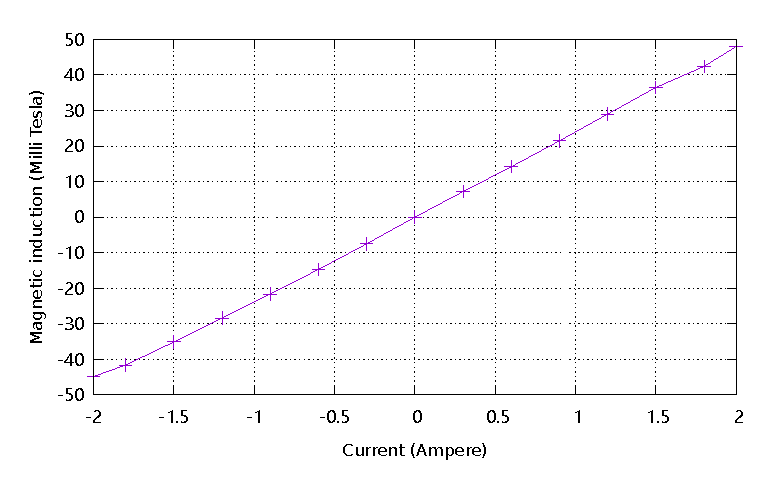
\includegraphics[width=0.9\linewidth]{../output/current-mfield.gnuplot}
\end{figure}
\newpage
\begin{table}[H]
    \centering
    \begin{tabular}{|c|c|c|c|c|c|c|c|c|c|}
        \hline
        检偏镜角度(${}^{\circ}$)  & 0   & 10  & 20  & 30  & 40  & 50  & 60  & 70  & 80  \\\hline
        光强($10^{-7} \si{A}$) & 13.73 & 1.25 & 15.13 & 58.60 & 119.30 & 203.00 & 289.00 & 375.00 & 440.00 \\\hline
        检偏镜角度(${}^{\circ}$)  & 90  & 100 & 110 & 120 & 130 & 140 & 150 & 160 & 170 \\\hline
        光强($10^{-7} \si{A}$) & 484.00 & 498.00 & 483.00 & 441.00 & 374.00 & 286.00 & 203.00 & 118.00 & 54.10 \\\hline
        检偏镜角度(${}^{\circ}$)  & 180 & 190 & 200 & 210 & 220 & 230 & 240 & 250 & 260 \\\hline
        光强($10^{-7} \si{A}$) & 14.18 & 0.69 & 16.20 & 58.00 & 123.80 & 197.20 & 284.00 & 362.00 & 421.00 \\\hline
        检偏镜角度(${}^{\circ}$)  & 270 & 280 & 290 & 300 & 310 & 320 & 330 & 340 & 350 \\\hline
        光强($10^{-7} \si{A}$) & 461.00 & 472.00 & 454.00 & 414.00 & 349.00 & 271.00 & 186.50 & 110.60 & 53.30 \\\hline
    \end{tabular}
    \caption{检偏器角度与光强关系,特定励磁电流$I=2.00 \si{A}$}
\end{table}
\begin{figure}[H]
    \centering
    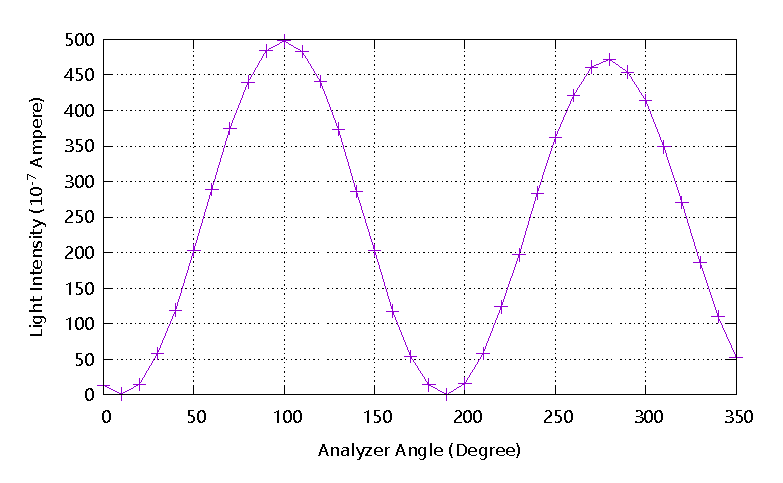
\includegraphics[width=0.9\linewidth]{../output/analyzer-angle-light-intensity-1.gnuplot}
\end{figure}
\newpage
\begin{table}[H]
    \centering
    \begin{tabular}{|c|c|c|c|c|c|c|c|c|c|}
        \hline
        检偏镜角度(${}^{\circ}$)  & 0   & 10  & 20  & 30  & 40  & 50  & 60  & 70  & 80  \\\hline
        光强($10^{-7} \si{A}$) & 15.53 & 1.44 & 17.20 & 58.10 & 121.50 & 199.50 & 290.00 & 372.00 & 440.00 \\\hline
        检偏镜角度(${}^{\circ}$)  & 90  & 100 & 110 & 120 & 130 & 140 & 150 & 160 & 170 \\\hline
        光强($10^{-7} \si{A}$) & 485.00 & 499.00 & 483.00 & 438.00 & 377.00 & 289.00 & 204.00 & 102.60 & 57.80 \\\hline
        检偏镜角度(${}^{\circ}$)  & 180 & 190 & 200 & 210 & 220 & 230 & 240 & 250 & 260 \\\hline
        光强($10^{-7} \si{A}$) & 15.73 & 1.30 & 16.35 & 57.50 & 122.80 & 204.00 & 282.00 & 361.00 & 421.00 \\\hline
        检偏镜角度(${}^{\circ}$)  & 270 & 280 & 290 & 300 & 310 & 320 & 330 & 340 & 350 \\\hline
        光强($10^{-7} \si{A}$) & 463.00 & 474.00 & 458.00 & 418.00 & 352.00 & 275.00 & 184.80 & 114.20 & 54.10 \\\hline
    \end{tabular}
    \caption{检偏器角度与光强关系,特定励磁电流$I=-2.00 \si{A}$}
\end{table}
\begin{figure}[H]
    \centering
    \includegraphics[width=0.9\linewidth]{../output/analyzer-angle-light-intensity-2.gnuplot}
\end{figure}
\newpage
\begin{table}[H]
    \centering
    \begin{tabular}{|c|c|c|c|c|c|c|c|c|c|}
        \hline
        检偏镜角度(${}^{\circ}$)  & 0   & 10  & 20  & 30  & 40  & 50  & 60  & 70  & 80  \\\hline
        光强($10^{-7} \si{A}$) & 44.00 & 18.35 & 4.82 & 7.37 & 25.70 & 58.10 & 101.20 & 150.70 & 196.40 \\\hline
        检偏镜角度(${}^{\circ}$)  & 90  & 100 & 110 & 120 & 130 & 140 & 150 & 160 & 170 \\\hline
        光强($10^{-7} \si{A}$) & 240.00 & 268.00 & 283.00 & 280.00 & 261.00 & 225.00 & 179.10 & 132.10 & 86.70 \\\hline
        检偏镜角度(${}^{\circ}$)  & 180 & 190 & 200 & 210 & 220 & 230 & 240 & 250 & 260 \\\hline
        光强($10^{-7} \si{A}$) & 48.20 & 18.29 & 4.34 & 7.48 & 26.10 & 59.30 & 100.30 & 141.50 & 190.10 \\\hline
        检偏镜角度(${}^{\circ}$)  & 270 & 280 & 290 & 300 & 310 & 320 & 330 & 340 & 350 \\\hline
        光强($10^{-7} \si{A}$) & 229.00 & 255.00 & 267.00 & 263.00 & 247.00 & 214.00 & 174.20 & 128.60 & 86.50 \\\hline
    \end{tabular}
    \caption{检偏器角度与光强关系,特定励磁电流$I=2.00 \si{A}$}
\end{table}
\begin{figure}[H]
    \centering
    \includegraphics[width=0.9\linewidth]{../output/analyzer-angle-light-intensity-3.gnuplot}
\end{figure}
\newpage
\begin{table}[H]
    \centering
    \begin{tabular}{|c|c|c|c|c|c|c|c|c|c|}
        \hline
        检偏镜角度(${}^{\circ}$)  & 0   & 10  & 20  & 30  & 40  & 50  & 60  & 70  & 80  \\\hline
        光强($10^{-7} \si{A}$) & 4.55 & 17.82 & 46.30 & 85.40 & 131.50 & 180.50 & 227.00 & 262.00 & 282.00 \\\hline
        检偏镜角度(${}^{\circ}$)  & 90  & 100 & 110 & 120 & 130 & 140 & 150 & 160 & 170 \\\hline
        光强($10^{-7} \si{A}$) & 285.00 & 272.00 & 242.00 & 201.00 & 150.10 & 100.90 & 60.70 & 26.20 & 7.25 \\\hline
        检偏镜角度(${}^{\circ}$)  & 180 & 190 & 200 & 210 & 220 & 230 & 240 & 250 & 260 \\\hline
        光强($10^{-7} \si{A}$) & 4.24 & 15.33 & 45.10 & 85.30 & 130.60 & 176.60 & 218.00 & 250.00 & 267.00 \\\hline
        检偏镜角度(${}^{\circ}$)  & 270 & 280 & 290 & 300 & 310 & 320 & 330 & 340 & 350 \\\hline
        光强($10^{-7} \si{A}$) & 268.00 & 255.00 & 226.00 & 185.50 & 139.90 & 95.20 & 53.50 & 23.20 & 7.25 \\\hline
    \end{tabular}
    \caption{检偏器角度与光强关系,特定励磁电流$I=-2.00 \si{A}$}
\end{table}
\begin{figure}[H]
    \centering
    \includegraphics[width=0.9\linewidth]{../output/analyzer-angle-light-intensity-4.gnuplot}
\end{figure}
\newpage
\begin{table}[H]
    \centering
    \begin{tabular}{|c|c|c|c|c|c|c|c|c|}
        \hline
        正向电流(A)              & 0.00 & 0.30 & 0.60 & 0.90 & 1.20 & 1.50 & 1.80 & 2.00 \\\hline
        检偏器角度$({}^{\circ})$  & 8.00 & 12.00 & 13.00 & 16.00 & 17.00 & 19.00 & 21.00 & 23.00 \\\hline
        反向电流(A)              & 0.00 & -0.30 & -0.60 & -0.90 & -1.20 & -1.50 & -1.80 & -2.00 \\\hline
        检偏器角度$({}^{\circ})$  & 8.00 & 5.00 & 3.00 & 2.00 & 0.00 & -1.00 & -4.00 & -5.00 \\\hline
        法拉第偏转角$({}^{\circ})$ & 0.00 & 3.50 & 5.00 & 7.00 & 8.50 & 10.00 & 12.50 & 14.00 \\\hline
    \end{tabular}
    \caption{检偏器角度与励磁电流关系}
\end{table}
\begin{figure}[H]
    \centering
    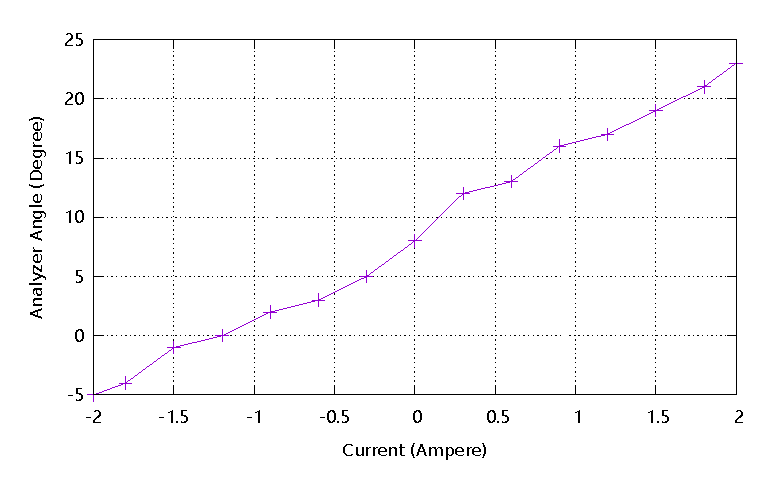
\includegraphics[width=0.9\linewidth]{../output/light-intensity-analyzer-angle.gnuplot}
\end{figure}
\newpage
\begin{table}[H]
    \centering
    \begin{tabular}{|c|c|c|c|c|c|c|c|c|}
        \hline
        $I/(\si{mA})$   & 0.00 & 5.00 & 10.00 & 15.00 & 20.00 & 25.00 & 30.00 & 35.00 \\\hline
        $U / (\si{V})$  & 1.40 & 1.60 & 1.70 & 1.70 & 1.70 & 1.80 & 1.80 & 1.80 \\\hline
        $P / (\si{mW})$ & 0.00 & 1.23 & 2.48 & 3.65 & 4.75 & 5.73 & 6.64 & 7.49 \\\hline
    \end{tabular}
    \caption{LED,温度$T=25.00{}^{\circ}C$,红色}
\end{table}
\begin{figure}[H]
    \centering
    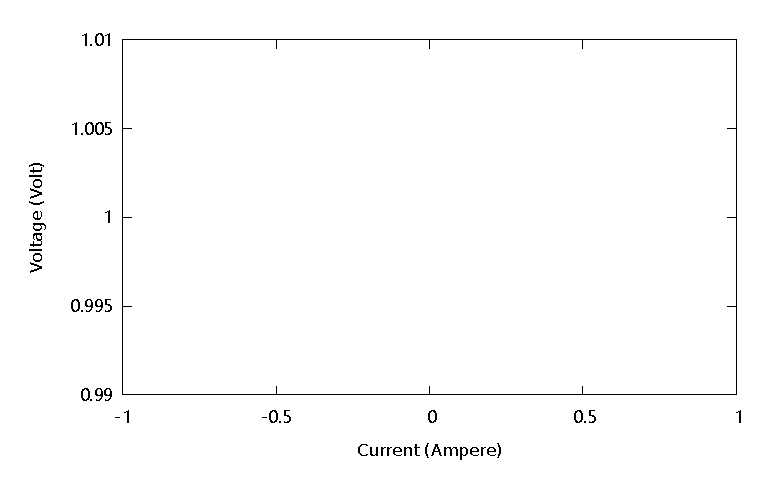
\includegraphics[width=0.9\linewidth]{../output/led-vc-1.gnuplot}
\end{figure}
\begin{figure}[H]
    \centering
    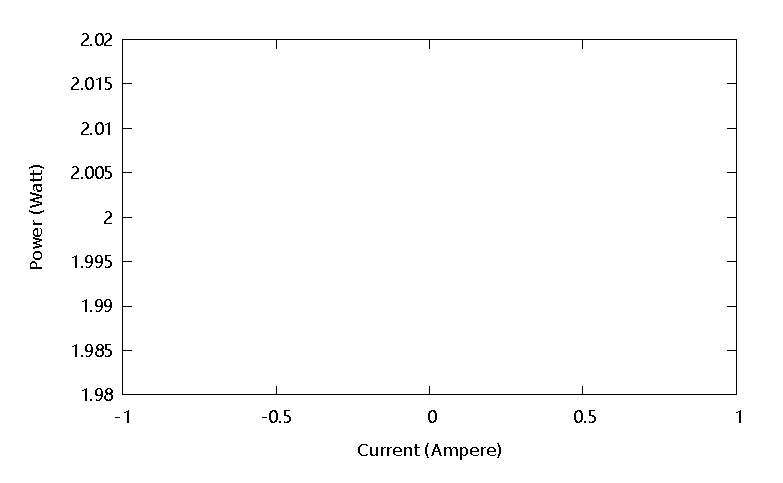
\includegraphics[width=0.9\linewidth]{../output/led-pc-1.gnuplot}
\end{figure}
\newpage
\begin{table}[H]
    \centering
    \begin{tabular}{|c|c|c|c|c|c|c|c|c|}
        \hline
        $I/(\si{mA})$   & 0.00 & 10.00 & 20.00 & 30.00 & 40.00 & 50.00 & 60.00 & 70.00 \\\hline
        $U / (\si{V})$  & 2.70 & 3.10 & 3.10 & 3.20 & 3.30 & 3.30 & 3.40 & 3.40 \\\hline
        $P / (\si{mW})$ & 0.00 & 2.89 & 5.52 & 7.54 & 9.13 & 10.22 & 10.30 & 11.03 \\\hline
    \end{tabular}
    \caption{LED,温度$T=25.00{}^{\circ}C$,紫色}
\end{table}
\begin{figure}[H]
    \centering
    \includegraphics[width=0.9\linewidth]{../output/led-vc-2.gnuplot}
\end{figure}
\begin{figure}[H]
    \centering
    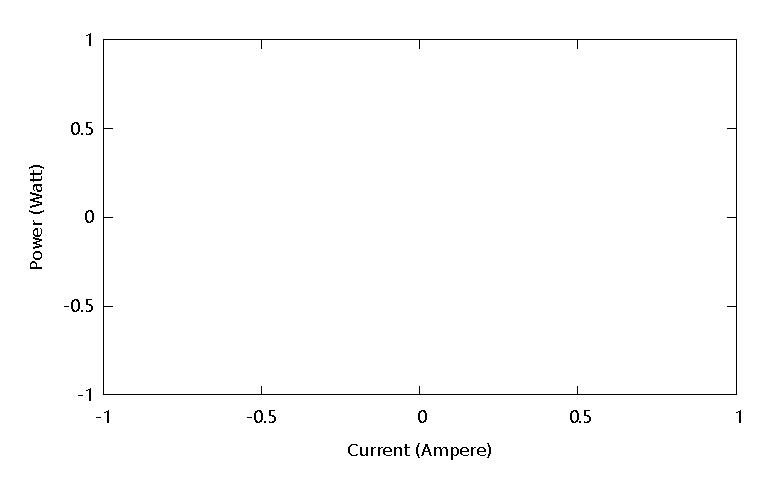
\includegraphics[width=0.9\linewidth]{../output/led-pc-2.gnuplot}
\end{figure}
\newpage
\begin{table}[H]
    \centering
    \begin{tabular}{|c|c|c|c|c|c|c|c|c|}
        \hline
        $I/(\si{mA})$   & 0.00 & 10.00 & 20.00 & 30.00 & 40.00 & 50.00 & 60.00 & 70.00 \\\hline
        $U / (\si{V})$  & 1.60 & 1.90 & 2.00 & 2.00 & 2.00 & 2.00 & 2.00 & 2.00 \\\hline
        $P / (\si{mW})$ & 0.00 & 1.24 & 2.31 & 3.05 & 3.48 & 3.61 & 3.40 & 3.33 \\\hline
    \end{tabular}
    \caption{LED,温度$T=25.00{}^{\circ}C$,黄色}
\end{table}
\begin{figure}[H]
    \centering
    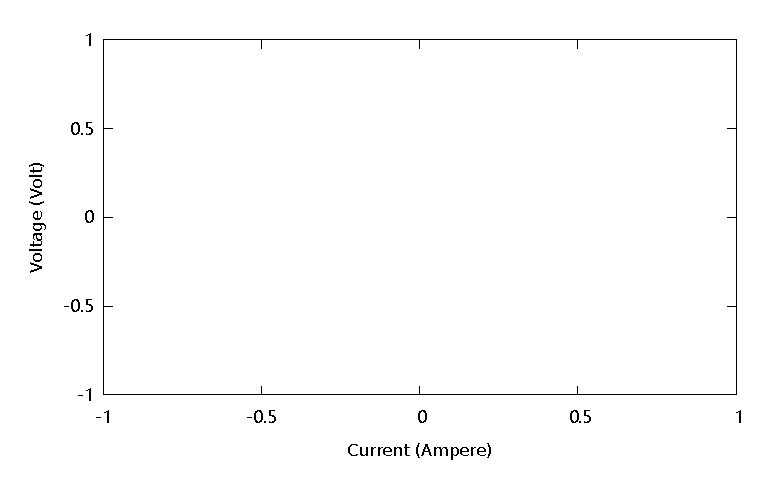
\includegraphics[width=0.9\linewidth]{../output/led-vc-3.gnuplot}
\end{figure}
\begin{figure}[H]
    \centering
    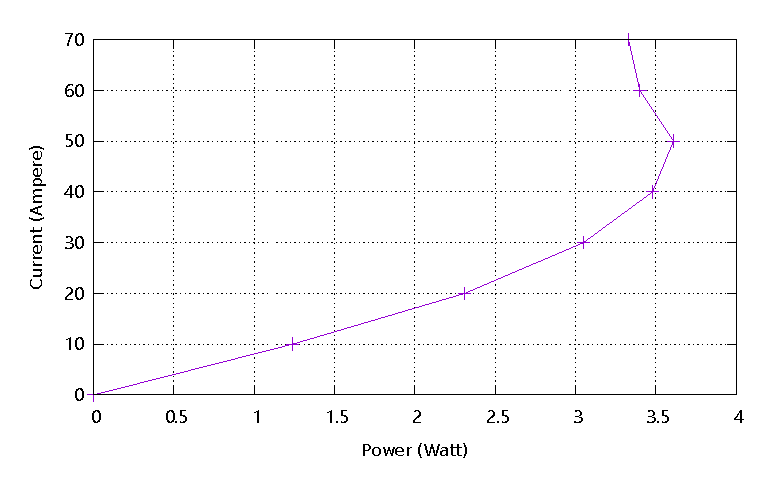
\includegraphics[width=0.9\linewidth]{../output/led-pc-3.gnuplot}
\end{figure}
\newpage
\begin{table}[H]
    \centering
    \begin{tabular}{|c|c|c|c|c|c|c|c|c|}
        \hline
        $I/(\si{mA})$   & 0.00 & 10.00 & 20.00 & 30.00 & 40.00 & 50.00 & 60.00 & 70.00 \\\hline
        $U / (\si{V})$  & 2.10 & 2.70 & 2.90 & 3.00 & 3.10 & 3.20 & 3.30 & 3.50 \\\hline
        $P / (\si{mW})$ & 0.00 & 6.54 & 9.79 & 12.12 & 13.81 & 14.71 & 15.86 & 17.52 \\\hline
    \end{tabular}
    \caption{LED,温度$T=25.00{}^{\circ}C$,绿色}
\end{table}
\begin{figure}[H]
    \centering
    \includegraphics[width=0.9\linewidth]{../output/led-vc-4.gnuplot}
\end{figure}
\begin{figure}[H]
    \centering
    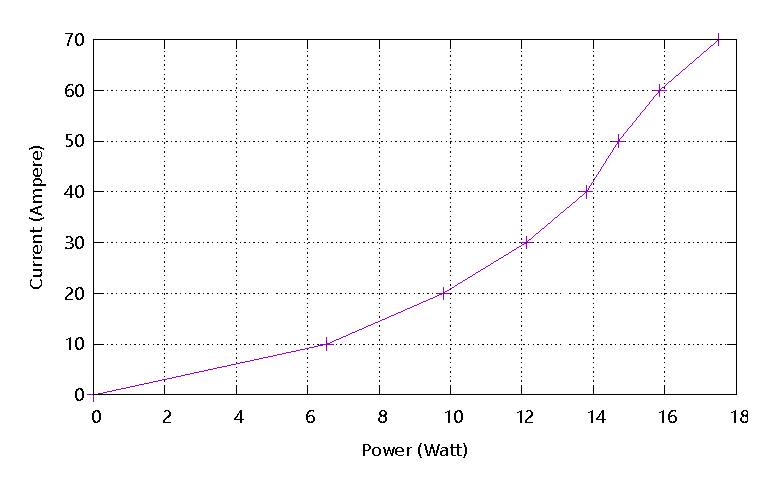
\includegraphics[width=0.9\linewidth]{../output/led-pc-4.gnuplot}
\end{figure}
\newpage
\begin{table}[H]
    \centering
    \begin{tabular}{|c|c|c|c|c|c|c|c|c|}
        \hline
        $I/(\si{mA})$   & 0.00 & 5.00 & 10.00 & 15.00 & 20.00 & 25.00 & 30.00 & 35.00 \\\hline
        $U / (\si{V})$  & 1.40 & 1.60 & 1.70 & 1.70 & 1.70 & 1.70 & 1.80 & 1.80 \\\hline
        $P / (\si{mW})$ & 0.00 & 1.89 & 3.88 & 5.67 & 7.48 & 8.92 & 10.29 & 11.47 \\\hline
    \end{tabular}
    \caption{LED,温度$T=35.00{}^{\circ}C$,红色}
\end{table}
\begin{figure}[H]
    \centering
    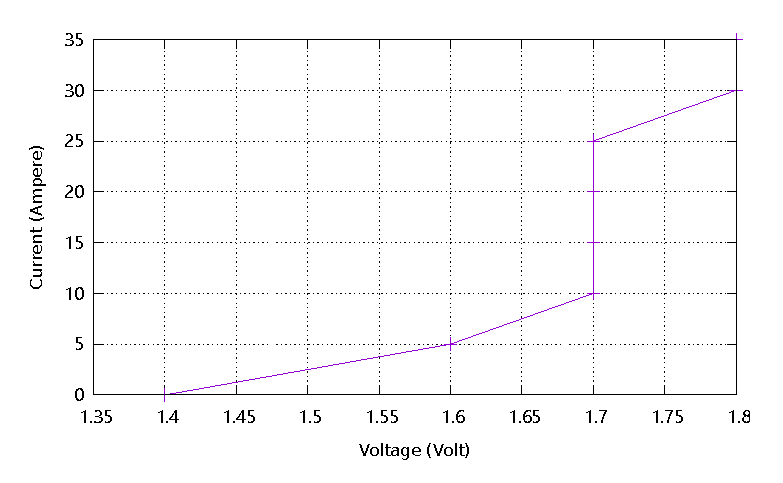
\includegraphics[width=0.9\linewidth]{../output/led-vc-5.gnuplot}
\end{figure}
\begin{figure}[H]
    \centering
    \includegraphics[width=0.9\linewidth]{../output/led-pc-5.gnuplot}
\end{figure}
\newpage
\begin{table}[H]
    \centering
    \begin{tabular}{|c|c|c|c|c|c|c|c|c|}
        \hline
        $I/(\si{mA})$   & 0.00 & 5.00 & 10.00 & 15.00 & 20.00 & 25.00 & 30.00 & 35.00 \\\hline
        $U / (\si{V})$  & 1.40 & 1.60 & 1.70 & 1.70 & 1.70 & 1.70 & 1.80 & 1.80 \\\hline
        $P / (\si{mW})$ & 0.00 & 1.82 & 3.65 & 5.45 & 7.04 & 8.45 & 9.77 & 10.91 \\\hline
    \end{tabular}
    \caption{LED,温度$T=45.00{}^{\circ}C$,红色}
\end{table}
\begin{figure}[H]
    \centering
    \includegraphics[width=0.9\linewidth]{../output/led-vc-6.gnuplot}
\end{figure}
\begin{figure}[H]
    \centering
    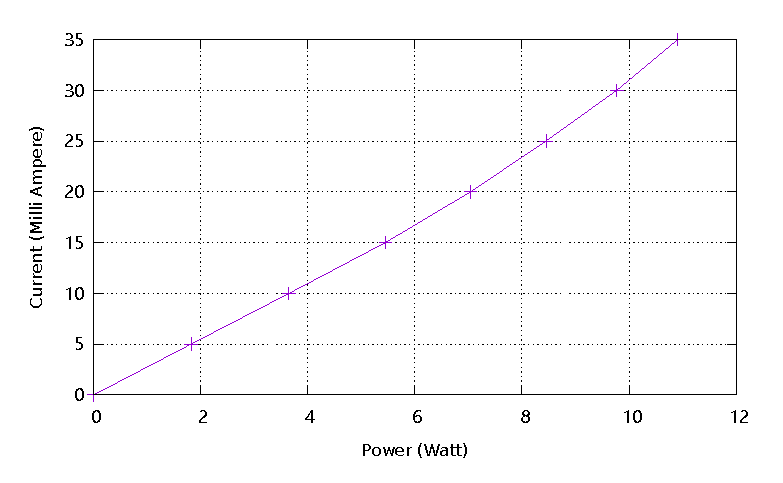
\includegraphics[width=0.9\linewidth]{../output/led-pc-6.gnuplot}
\end{figure}
\newpage
\begin{table}[H]
    \centering
    \begin{tabular}{|c|c|c|c|c|c|c|c|c|}
        \hline
        $I/(\si{mA})$   & 0.00 & 5.00 & 10.00 & 15.00 & 20.00 & 25.00 & 30.00 & 35.00 \\\hline
        $U / (\si{V})$  & 1.40 & 1.60 & 1.70 & 1.70 & 1.70 & 1.70 & 1.80 & 1.80 \\\hline
        $P / (\si{mW})$ & 0.00 & 1.72 & 3.44 & 5.10 & 6.55 & 8.01 & 9.23 & 10.34 \\\hline
    \end{tabular}
    \caption{LED,温度$T=55.00{}^{\circ}C$,红色}
\end{table}
\begin{figure}[H]
    \centering
    \includegraphics[width=0.9\linewidth]{../output/led-vc-7.gnuplot}
\end{figure}
\begin{figure}[H]
    \centering
    \includegraphics[width=0.9\linewidth]{../output/led-pc-7.gnuplot}
\end{figure}
\newpage
\begin{table}[H]
    \centering
    \begin{tabular}{|c|c|c|c|c|c|c|c|c|}
        \hline
        $I/(\si{mA})$   & 0.00 & 5.00 & 10.00 & 15.00 & 20.00 & 25.00 & 30.00 & 35.00 \\\hline
        $U / (\si{V})$  & 1.40 & 1.60 & 1.60 & 1.70 & 1.70 & 1.70 & 1.70 & 1.80 \\\hline
        $P / (\si{mW})$ & 0.00 & 1.56 & 3.20 & 4.71 & 6.17 & 7.49 & 8.65 & 9.67 \\\hline
    \end{tabular}
    \caption{LED,温度$T=65.00{}^{\circ}C$,红色}
\end{table}
\begin{figure}[H]
    \centering
    \includegraphics[width=0.9\linewidth]{../output/led-vc-8.gnuplot}
\end{figure}
\begin{figure}[H]
    \centering
    \includegraphics[width=0.9\linewidth]{../output/led-pc-8.gnuplot}
\end{figure}
\newpage


\section{参考文献}
\begin{itemize}[leftmargin=0pt]
    \item[] 综合物理实验讲义
\end{itemize}
\end{document}